%---Linda

The post processing is based on the correction of the raw data.
Firstly, we have to process the data with the corresponding data of the base station data to get a higher accurancy of the GPS data.
The nearest base station is Statens Kartverks SatRef located on Platåberget with a distance between 14 km and 20 km depending on the mass balance stake.
In the following the mass balance stake is only named stake and the pole with the rover will be shortend to the name rover.
\medskip

In the previous reports the post processing was done with the commercial software Trimble Business Center (TBC). 
In our report we use a new method for the postprocessing. 
This method is an open source (OS) alternative which is available for different system softwares. 
The TBC is only available on a windows system and needs a licens. 
We operate both methods to compare the results of both methods.
\medskip

\subsection{Trimble}

While the post processing with the usual method in the TBC all steps from section 5 in Gölles (2012) are done.
For each day the data file from the measurements and the corresponding base station data file is imported. 
We have data for the days of year (doy) 070, 072, 074 and 075.
All files from the base station are in the .o18-format. 
The data from the reciever have the .t02 format. 
After the post processing the results from the are stored in a .csv-file.
The GNSS processing in the TBC used the combination of reference and rover data.
The goal is “fix” the number of whole wavelengths between the rover and satellites.
This process is done in two steps by generating a 'float' solution an and resolve an integer value. 
Wheh it is sucessful the solution is defined as 'fixed'.
The transition from 'float' to 'fixed' is the initialization.
A slow convergence of the solution is possible for longer baselines or shielding of the signal by objects in the surrounding.
By mistake it is possible that during the post processing process a wrong fixed values is hold which can lead to an unnormal high position error.
After some amount of time the float solution can switch instantaneously to a fixed solution. 
There is also a disadvantag of the float and fixed approach for integer ambiguity resolution.
At some point in time the convergence to fixed solution is hold on and impossible to change. 
The result define then a wrong position, which is caused by a incorrect set of interger ambiguties.
The TBC use automatically the best way to process the position data. 
It is distingushed in short and long baselines.
Baselines are determined by the distance between rover and reference station.
For longer baselines the errors have to be reduced with an additional approach like a model.
For different settings and situations the TBC used different approaches for the tropospheric and ionospheric errors and choose the right combinaion of different applications.
This makes it difficult to distinguish the settings used for the post processing to compare with the open source processing \citep{Trprocess}.
\medskip

\subsection{Open source}
The OS post processing requires different processing steps.
First of all the raw data file has to be transformed from the original Trimble format .t02 to the .tdg-format, because .t02-files are not readable for the final post processing program.
This transformation was done with the programm runpkr00 which is available on the website of unavco \url{http://kb.unavco.org/kb/article/trimble-runpkr00-v5-40-latest-version-mac-osx-10-7-windows-xp-7-linux-solaris-744.html}.
The used command is 
\begin{verbatim} 
runpkr00 -g -d filename.t02 
\end{verbatim}.
Due to problems with the package we had to do a manual transformation of the package.
To provide the correct file format for the last post processing step we use the toolkit teqc.
This toolkit is also available on the website of unavco \url{https://www.unavco.org/software/data-processing/teqc/teqc.html}.
Then the file can be converted by another commad using
\begin{verbatim}
./teqc +nav filename.nav +obs filename.obs filename.tgd
\end{verbatim} 
to an observation (.obs) and navigation (.nav) file.
After that it is necessary to download also the base station data from the platform \url{http://ftp.statkart.no/}.
The final step in the post processing of the GPS data is done with the open source program package \textit{RTKLIB}.
This package is available for the download in the website \url{http://www.rtklib.com/rtklib.htm}.
In this package we use the executable rtkpost.exe in the subdirectory \textit{/bin} of the downloaded full package with source Programs with the version 2.4.2.
In this software the two navigation file from the receiver and the base station as well as the observation file from the receiver has to be read in.
For this method the .n18-format from the basestation is needed as comparable navigation file.
The next steps are consistent to the description on the website \url{https://docs.emlid.com/reach/common/tutorials/gps-post-processing/}.
For this we had to modify the settings of rtkpost.exe and load the three required files. 
The final output after the post processing is a position file (.pos). 
This file includes for every time step the post processed position in longitude and latitude.
Then we calculate a median over all time steps to get an average position for every measurement.
Because we consistenly use the UTM coordinate system, we transform the lon/lat coordinates by using a python function.
All the analysis in this report is made with python.
\medskip

% therory of the open source post processing
The header with the settings for the OS post processing is available in the appendix.
The setting are as similar as possible to the TBC settings.
But like described is the processing method in the TBC flexible.
In the open source post processing it is possible to select different correction methods for the tropospheric and ionospheric correction. 
Due to missing informations from TBC the probaly best method was choosen with 'broadcast' correction for the ionosphere and the 'saastamoinen' correction for optimize the accurancy due to tropospheric errors. 
The other settings can be taken from the header information to repeat the OS post processing. 
\medskip

The results of the OS post processing are given as a time series of latitude, longitude and elevation, where the horizontal components are transformed to the UTM coordinate system. 
For the better understanding of the OS values it is usefull to compare timeseries of the post processed positions for two different measurements at the same stake.
For both stakes the settings in the post processing were the same.
In the first measurement (figure \label{GPS:fig:T1-i_timeseries}) the values coverge after a few seconds to a fixed solution.
In the second measurement (figure \label{GPS:fig:T1-ii_timeseries}) the values vary during the hole time series.
Out of this time series the weighted average was calculated to get one position value for every stake, the OS value.
The properties of the second measurement leads to a bigger difference between the TBC value and the OS value.
A comparison to the time series of the TBC post processing is not possible, because it is not possible to get this out of the TBC.

\begin{figure}[H]
    \centering
    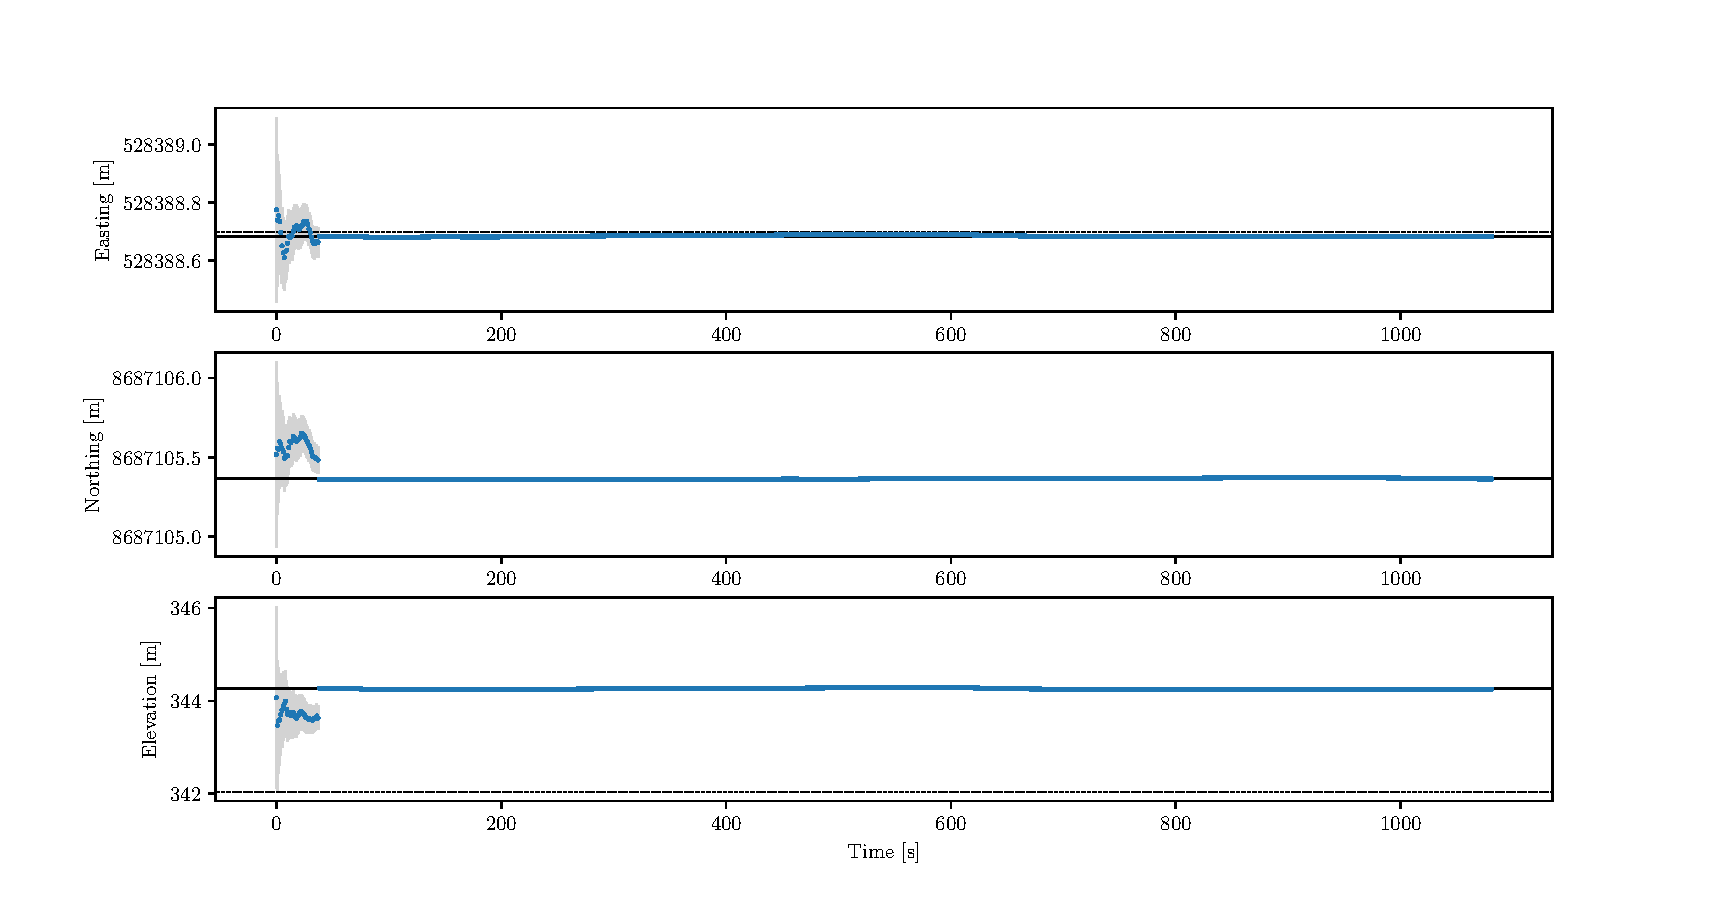
\includegraphics[width=\textwidth]{./figs/timeseries/46250700_corr-T1-i-2017_Timeseries-east-north-elev.pdf}
    \caption{First of two 15 minutes measurements of position of stake T1-2017.}
    \label{GPS:fig:T1-i_timeseries}
\end{figure}

\begin{figure}[H]
    \centering
    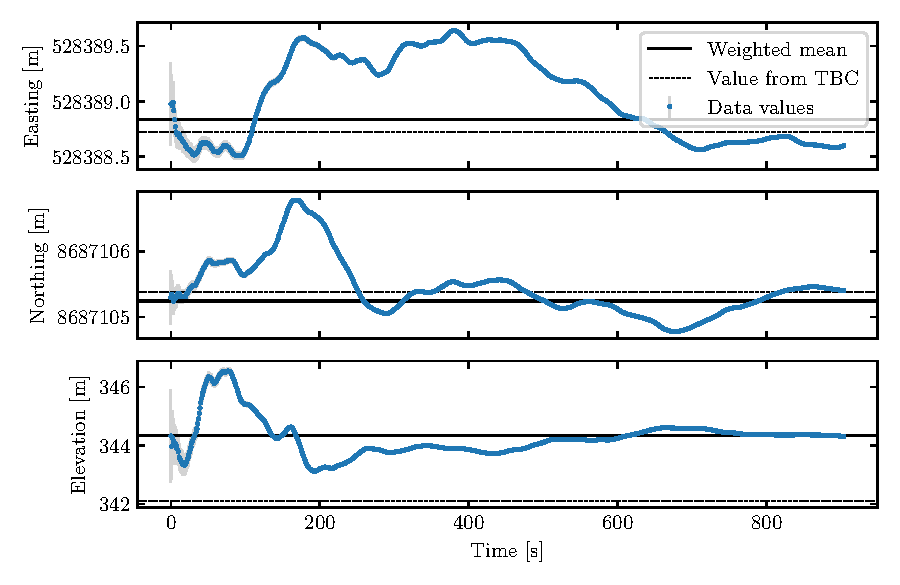
\includegraphics[width=\textwidth]{./figs/timeseries/46250723_corr-T1-ii-2017_Timeseries-east-north-elev.pdf}
    \caption{Second 15 minutes measurement of position of stake T1-2017.}
    \label{GPS:fig:T1-ii_timeseries}
\end{figure}


\subsection{Stake correction}
The post processed data with the base station data are not the final data. 
To get the final, we have to make the stake correction include the different aspects from our measurement setup (see section setup).
We subtract the distance between the rover and the stake from the northing component.
Also it was necessary to correct the position on the ice surface with the inclination of the stake. 
For this, we consider the inclination of the stake and calculate the error dependent on the height of the stake and the direction of the inclination.
The raw data from our measurements which are relevant for our stake corrections are in the appendix in table \ref{GPS:tab:fb_others_tab}.
For the better understanding all variables for the stake corrections are shown in the schematic figure \ref{GPS:fig:schema}.
\medskip

\begin{figure}[H]
	\centering
	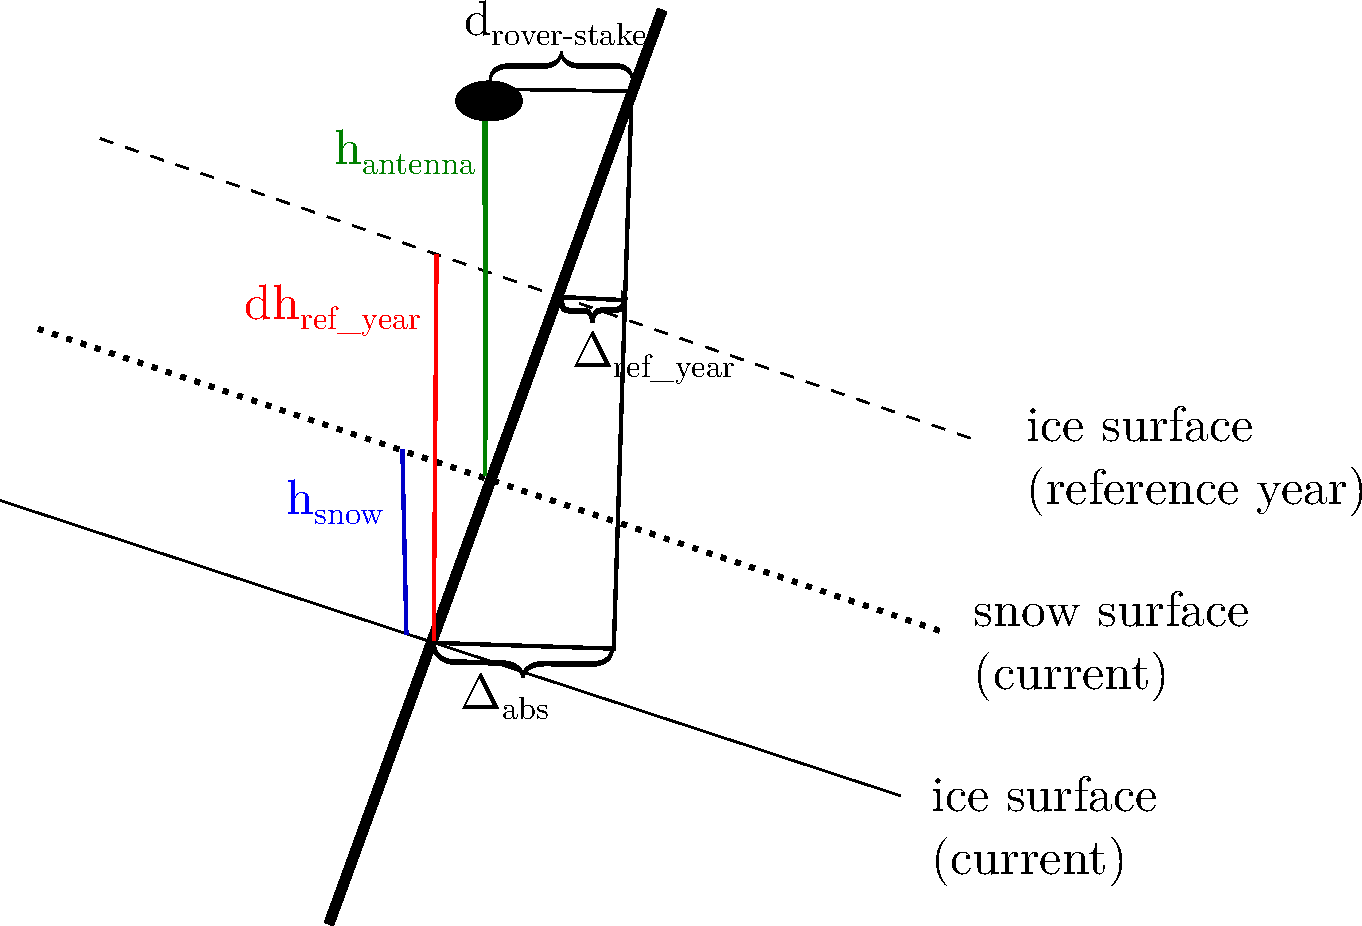
\includegraphics[width=0.9\linewidth]{./figs/pictures/schematic_setup.pdf}
	\caption{Schematic figure of the relevant parameter in the measurment setup.}
	\label{GPS:fig:schema}
\end{figure}

The stake correction is derived by the geomatry of our measurement setup.
First the absolut horizontal difference $\Delta_{\text{abs}}$ depending in the inclination $\alpha$ and the height composite of snow depth $h_{\text{snow}}$ and antenna height $h_{\text{antenna}}$.
\begin{equation}
	\Delta_{\text{abs}} = (h_{\text{snow}} + h_{\text{antenna}}) * sin(\alpha)
\end{equation}

Then the correction is different for the northing and easting. The norting correction is calculated with the cosinus of the direction of the inclination $\phi$. 
The angle of direction is defined in a range from 0$^{\circ}$ to 359$^{\circ}$ with 0$^{\circ}$ for North, 90$^{\circ}$ for East, 180$^{\circ}$ for South and 270$^{\circ}$ for West.
Due to geometrical reasons the sign has to be negative. 
Additionally the the distance between the rover and the stake $d_{\text{rover-stake}}$ has to be subtracted from the original northing.
\begin{equation}
	\Delta_{\text{north}} = - (\Delta_{\text{abs}} * cos(\phi)) - d_{\text{rover-stake}}
\end{equation}

The easting difference $\Delta_{\text{east}}$ is calculated with the sine of $\phi$.
\begin{equation}
	\Delta_{\text{east}} = - \Delta_{\text{abs}} * sin(\phi)
\end{equation}

The elevation correction is different between the OS and the TCS values.
For the TBC values the elevation correction $\Delta_{\text{elev,TBC}}$ only the $h_{\text{snow}}$ need to be subtracted because the $h_{\text{antenna}}$ is already caluclated out while the measurement with the Controller.
\begin{equation}
	\Delta_{\text{elev,TBC}} = - h_{\text{snow}} 
\end{equation}

The elevation correction of the OS elevation $\Delta_{\text{elev,os}}$ is done by $h_{\text{snow}}$ and $h_{\text{antenna}}$.
\begin{equation}
	\Delta_{\text{elev,os}} = - (h_{\text{snow}} + h_{\text{antenna}}) 
\end{equation}

\subsubsection*{Referenced positions}

To calculate the actual velocity it is necessary to reference the location of the stake to the ice surface elevation of the referenced year. 
This has been done for the years 2015, 2016 and 2017 on the 2018 OS values.
In gerneal, the calculation works in the similar way.
The height for stake correction with the inclination is different, because the relevant height difference is, in our case of an over all ablation, lower than for the actual values of this year. So the height difference of the height surface between the referenced year and 2018 $dh_{year,2018}$ is considered for the calculation of the absolute horizontal difference $\Delta_{year,2018}$.

\begin{equation}
	\Delta_{year,2018} = (h_{\text{snow}} + h_{\text{antenna}} - dh_{year,2018}) * sin(\alpha)
\end{equation}

\subsection{Evaluation}

For the difference between the two different methods is not systematic and in the avereage of the absolute values in the order of centimeters with 0.09 m for the northing, 0.05 m for thehe  easting and 0.24 m for the elevation. This is mainly caused by a few unclear values after the post processing. The meadian of the northing and eastind difference is about 0.01 m and for the elevation only 0.07 m. For the comparison the TBC post processed coordinates are in the appendix in table \ref{GPS:tab:tbc_tab}.
The differences for northing, easting and elevation for every stake is displayed in a table in the appendix in table \ref{GPS:tab:diff_tab}. 

This shows that the OS processed values are a reasonable replacement for the TBC values.
This means that in the following report the OS values are consideres.
This means also that the error propagation is done for the OS values so we can finaly determine the uncertainty of the velocity values.

\subsection{Error propagation}

The calculations for the error propagation are done by following the common rule.
The accurancy of the post processed postions with the base station data is decreasing with a increasing distance to the base station. 
But this error is at least one order of magnitude smaller than the other errors. 
The other accurancies are determined by the quality of our measurements \ref{GPS:tab:errors}.

\begin{table}[H]
	\caption{Used error values for the error propagation.}
	\centering
	\begin{tabular}{lc}
	\toprule
        error &  value \\
	\midrule
    $ \delta_{\alpha} $ &  3$^{\circ}$ \\
    $ \delta_{\phi} $ &  22.5$^{\circ}$ \\
    $ \delta_{h_{snow}}$ &  0.02 m \\
    $ \delta_{h_{antenna}} $ &  0.05 m \\
    $ \delta_{dh_{year,2018}} $ &  0.10 m \\
    $ \delta_{d_{rover-stake}} $ &  0.02 m \\
    $ \overline{\delta_{\Delta_{north}}} $ & 0.40 m \\
    $ \overline{\delta_{\Delta_{east}}} $ & 0.19 m \\
    $ \overline{\delta_{\Delta_{elev}}} $ & 0.89 m \\
    \bottomrule
	\end{tabular}
	\label{GPS:tab:errors}
\end{table} 

The error calculation for the final position is dependent of different errors.

The error of the absolut horizontal difference $\delta_{\Delta_{\text{abs}}}$ is dependent on the errors of the parameter and the parameter itself.
\begin{equation}
	\delta_{\Delta_{\text{abs}}} = \sqrt{(h_{\text{snow}} + h_{\text{antenna}})^2 * \delta_{\alpha}^2 * cos^2(\alpha) + (\delta_{h_{\text{snow}}}^2 + \delta_{h_{\text{antenna}}}^2) * \sin^2(\alpha)}
\end{equation}

The error of the northing correction $\delta_{\Delta_{\text{north}}}$ is
\begin{equation}
	\delta_{\Delta_{\text{north}}} = \sqrt{\delta_{\Delta_{\text{abs}}}^2 * cos^2(\phi) + \Delta_{\text{abs}}^2 * \delta_{\phi}^2 * sin^2(\phi) + \delta_{d_{\text{rover-stake}}}^2}
\end{equation}

The error of the easting correction $\delta_{\Delta_{\text{east}}}$ is
\begin{equation}
	\delta_{\Delta_{\text{east}}} = \sqrt{\delta_{\Delta_{\text{abs}}}^2 * sin^2(\phi) + \Delta_{\text{abs}}^2 * \delta_{\phi}^2 * cos^2(\phi)}
\end{equation}

The error of the elevation correction $\delta_{\Delta_{\text{elev}}}$ is
\begin{equation}
\delta_{\Delta_{\text{elev}}} = \sqrt{\delta_{h_{\text{snow}}}^2 + \delta_{h_{\text{antenna}}}^2}
\end{equation}
	
Based on this errors the total error for norting $\delta_{\Delta_{\text{total,north}}}$, easting $\delta_{\Delta_{\text{total,east}}}$ and eleavtion $\delta_{\Delta_{\text{total,elev}}}$ can calculated with the error of the time series of our OS post processed GPS time series $\delta_{\Delta_{\text{ts,north}}}$ for northing, $\delta_{\Delta_{\text{ts,east}}}$ for easting and $\delta_{\Delta_{\text{ts,elev}}}$ for the elevation.
\begin{equation}
	\delta_{\Delta_{\text{total,north}}} = \sqrt{\delta_{\Delta_{\text{ts,north}}}^2 + \delta_{\Delta_{\text{north}}}^2}
\end{equation}

\begin{equation}
	\delta_{\Delta_{\text{total,east}}} = \sqrt{\delta_{\Delta_{\text{ts,east}}}^2 + \delta_{\Delta_{\text{east}}}^2}
\end{equation}

\begin{equation}
	\delta_{\Delta_{\text{total,elev}}} = \sqrt{\delta_{\Delta_{\text{ts,elev}}}^2 +\delta_{\Delta_{\text{elev}}}^2}
\end{equation}

\subsubsection*{Referenced positions}
For the refenced positions only two euations differ to the previous error propagation. 
The error of the absolute difference $\Delta_{year,2018}$ is
\begin{equation}
\begin{split}
\delta_{\Delta_{year,2018}} = & 
\ ((h_{\text{snow}} + h_{\text{antenna}} - dh_{year,2018})^2 * \delta_{\alpha}^2 * cos^2(\alpha)\\
&+ (\delta_{h_{\text{snow}}}^2 + \delta_{h_{\text{antenna}}}^2 + \delta_{dh_{year,2018}}^2) * \sin^2(\alpha))^{1/2}
\end{split}
\end{equation}

The error for the elevation correction $\delta_{\Delta_{year, \text{elev}}}$ is also different by the uncertainty of the height difference of the ice surface $\delta_{dh_{\text{year, 2018}}}$.
\begin{equation}
	\delta_{\Delta_{year, \text{elev}}} = \sqrt{\delta_{h_{\text{snow}}}^2 + \delta_{h_{\text{antenna}}}^2 + \delta_{dh_{\text{year, 2018}}}^2}
\end{equation}

\subsection{Final positions}

The final data with all the processing and correction included show the actual position of the stakes on this years ice surface.

\begin{table}[H]
	\caption{Final positions after the open source post processing and stake correction with the error.}
	\centering
	\begin{tabular}{lrrrrrr}
\toprule
        Name &  Northing [m] &  Error Northing [m] &  Easting [m] &  Error Easting [m] &  Elevation [m] &  Error Elevation [m] \\
\midrule
    BL2-2016 &    8686150.74 &                0.16 &    523049.41 &               0.11 &         436.89 &                 0.48 \\
    BL2-2018 &    8686149.82 &                0.01 &    523051.47 &               0.03 &         437.74 &                 0.06 \\
    BL3-2016 &    8686091.51 &                0.27 &    523544.75 &               0.13 &         490.82 &                 0.25 \\
    BL3-2018 &    8686091.17 &                0.42 &    523545.34 &               0.10 &         491.39 &                 1.03 \\
    BL4-2018 &    8686098.58 &                0.17 &    524179.27 &               0.15 &         573.74 &                 0.20 \\
  BL4-i-2016 &    8686098.47 &                0.26 &    524179.80 &               0.19 &         571.65 &                 0.20 \\
 BL4-ii-2016 &    8686098.39 &                1.30 &    524179.92 &               0.31 &         571.36 &                 4.82 \\
  BL5-i-2017 &    8686130.74 &                0.09 &    524644.27 &               0.01 &         628.63 &                 0.09 \\
 BL5-ii-2017 &    8686130.74 &                0.28 &    524644.28 &               0.15 &         628.56 &                 0.75 \\
     T1-2018 &    8687106.55 &                0.32 &    528388.42 &               0.07 &         341.59 &                 0.24 \\
   T1-i-2017 &    8687105.69 &                0.13 &    528388.68 &               0.18 &         341.26 &                 0.12 \\
  T1-ii-2017 &    8687105.58 &                0.45 &    528388.84 &               0.44 &         341.38 &                 0.65 \\
     T2-2016 &    8687321.31 &                0.42 &    527951.88 &               0.14 &         394.88 &                 2.34 \\
     T2-2018 &    8687319.62 &                0.28 &    527951.35 &               0.27 &         395.86 &                 1.61 \\
   T2-i-2017 &    8687321.37 &                0.30 &    527950.58 &               0.25 &         395.22 &                 0.34 \\
  T2-ii-2017 &    8687320.98 &                1.31 &    527951.01 &               0.26 &         394.74 &                 1.26 \\
     T3-2017 &    8687273.11 &                0.11 &    527598.29 &               0.01 &         422.59 &                 0.07 \\
     T4-2016 &    8687138.56 &                0.47 &    527123.97 &               0.34 &         486.80 &                 1.07 \\
     T4-2018 &    8687137.72 &                1.05 &    527124.90 &               0.37 &         487.94 &                 2.33 \\
     T5-2016 &    8686938.28 &                0.57 &    526692.25 &               0.25 &         534.57 &                 0.72 \\
     T5-2018 &    8686937.68 &                0.21 &    526690.76 &               0.21 &         535.09 &                 0.45 \\
     T6-2016 &    8686675.01 &                0.51 &    526250.17 &               0.22 &         561.87 &                 0.89 \\
     T6-2018 &    8686674.78 &                0.48 &    526246.88 &               0.39 &         560.47 &                 0.79 \\
     T7-2015 &    8686578.89 &                0.24 &    525858.01 &               0.17 &         615.10 &                 0.71 \\
     T7-2017 &    8686579.37 &                0.19 &    525858.38 &               0.04 &         615.95 &                 0.71 \\
     T8-2017 &    8686471.52 &                0.48 &    525523.82 &               0.13 &         649.73 &                 1.02 \\
\bottomrule
\end{tabular}

	\label{GPS:tab:os_tab}
\end{table}
